\chapter{導論}
\label{c:1}

%==========================================================================================
\section{第一階層子標題}

各階層子標題均應置於左側,並於其下方不空行。

本規範為一般性規範,各所得依其學術領域之慣用格式,訂定相關規範。本規範為一般性規範,各所得依其學術領域之慣用格式,訂定相關規範。本規範為一般性規範,各所得依其學術領域之慣用格式,訂定相關規範。本規範為一般性規範,各所得依其學術領域之慣用格式,訂定相關規範。本規範為一般性規範,各所得依其學術領域之慣用格式,訂定相關規範。本規範為一般性規範,各所得依其學術領域之慣用格式,訂定相關規範。本規範為一般性規範,各所得依其學術領域之慣用格式,訂定相關規範。本規範為一般性規範,各所得依其學術領域之慣用格式,訂定相關規範。本規範為一般性規範,各所得依其學術領域之慣用格式,訂定相關規範。本規範為一般性規範,各所得依其學術領域之慣用格式,訂定相關規範。本規範為一般性規範,各所得依其學術領域之慣用格式,訂定相關規範。本規範為一般性規範,各所得依其學術領域之慣用格式,訂定相關規範。本規範為一般性規範,各所得依其學術領域之慣用格式,訂定相關規範。

%==========================================================================================
\subsection{第二階層子標題}

第二階層子標題之內文。

%==========================================================================================
\subsubsection{第三階層子標題}

第三階層子標題之內文。



%==========================================================================================
\section{Figure}
\label{ss:Figure}
\begin{figure}[htpb!]
  \centering
    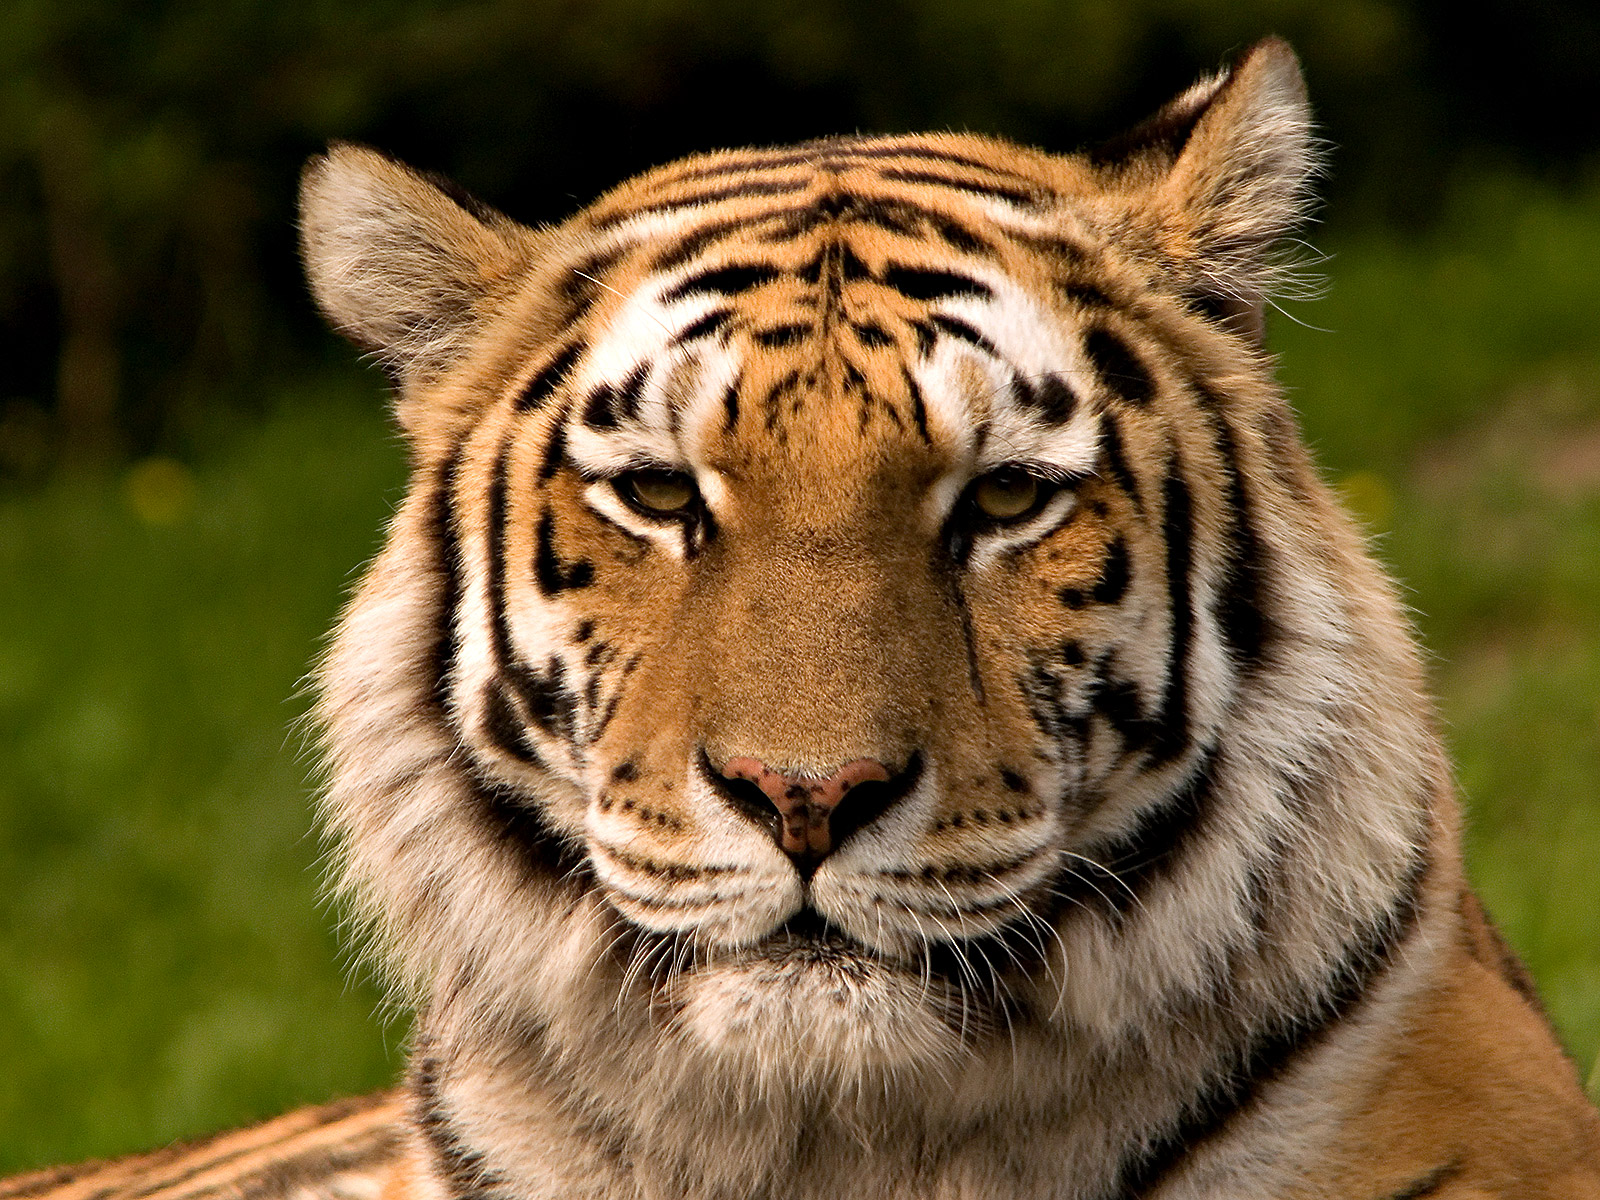
\includegraphics[width=0.5\textwidth]{fig/tiger.jpeg}
    \caption{\label{fig:tiger}A picture of a tiger.}
\end{figure}

Figure~\ref{fig:tiger} is a picture of a tiger.


% ntut



下圖\ref{fig:kamado}顯示的是 ``竈門炭治郎'' 的圖片。

\begin{figure}[h!]
    \centering
    
\includegraphics[width=0.85\textwidth]{fig/kamado/maxresdefault.jpg}
    \caption{這張圖片的說明, 竈門炭治郎。}
    \label{fig:kamado}
\end{figure}


竈門炭治郎的招式,是水之呼吸,見圖\ref{fig:kamado_ab}。圖\ref{fig:kamado_a}顯示的是 竈門炭治郎本人的圖片。圖\ref{fig:kamado_b}顯示的是 竈門炭治郎招式的圖片。


\begin{figure}[htbp]
\centering
\subfigure[我是圖a的說明]{
	
\includegraphics[width=0.22\textwidth]{fig/kamado/a.jpg}
	\label{fig:kamado_a}
}
\subfigure[我是圖b的說明]{
	
\includegraphics[width=0.22\textwidth]{fig/kamado/b.jpg}
	\label{fig:kamado_b}
}
\caption{我是整張圖a的說明}
\label{fig:kamado_ab}
\end{figure}



竈門炭治郎的招式,是水之呼吸,見圖\ref{fig:kamado_ab2}。圖\ref{fig:kamado_a2}顯示的是 竈門炭治郎本人的圖片。圖\ref{fig:kamado_b2}顯示的是 竈門炭治郎招式的圖片。圖\ref{fig:kamado_a3}顯示的是...。圖\ref{fig:kamado_b3}顯示的是...。



\begin{figure*}[htbp]
\centering
\subfigure[我是圖a的說明]{
	
\includegraphics[width=0.22\textwidth]{fig/kamado/a.jpg}
	\label{fig:kamado_a2}
}
\subfigure[我是圖b的說明]{
	
\includegraphics[width=0.22\textwidth]{fig/kamado/b.jpg}
	\label{fig:kamado_b2}
}
\subfigure[我是圖c的說明]{
	
\includegraphics[width=0.22\textwidth]{fig/kamado/a.jpg}
	\label{fig:kamado_a3}
}
\subfigure[我是圖d的說明]{
	
\includegraphics[width=0.22\textwidth]{fig/kamado/b.jpg}
	\label{fig:kamado_b3}
}
\caption{我是整張圖a的說明}
\label{fig:kamado_ab2}
\end{figure*}





中文缺字,。內文提到圖\ref{punica_compare}, Fig~\ref{punica_a}, Fig~\ref{punica_b}, Fig~\ref{punica_c}, Fig~\ref{punica_d}, Fig~\ref{punica_e}, Fig~\ref{punica_f}


\begin{figure}[htbp]
\centering
\subfigure[子圖a說明]{
	
\includegraphics[width=0.32\textwidth]{fig/flower/file(0).pdf}
	\label{punica_a}
}
\subfigure[子圖b說明]{
	
\includegraphics[width=0.32\textwidth]{fig/flower/file(1).pdf}
	\label{punica_b}
}
\subfigure[子圖c說明]{
	
\includegraphics[width=0.32\textwidth]{fig/flower/file(2).pdf}
	\label{punica_c}
}
\subfigure[子圖d說明]{
	
\includegraphics[width=0.32\textwidth]{fig/flower/file(3).pdf}
	\label{punica_d}
}
\subfigure[子圖e說明]{
	
\includegraphics[width=0.32\textwidth]{fig/flower/file(4).pdf}
	\label{punica_e}
}
\subfigure[子圖f說明]{
	
\includegraphics[width=0.32\textwidth]{fig/flower/file(4).pdf}
	\label{punica_f}
}
\caption{...}
\label{punica_compare}
\end{figure}




%==========================================================================================
\section{Table}
\label{ss:Table}

\href{http://en.wikibooks.org/wiki/LaTeX/Tables}{Table examples on WIKIBOOKS}.

\begin{table}[htpb]\begin{center}
\caption{Table Example 1}
\begin{tabularx}{8cm}{llX}
\hline
Start & End  & Character Block Name \\
\hline
3400  & 4DB5 & CJK Unified Ideographs Extension A \\
4E00  & 9FFF & CJK Unified Ideographs \\
\hline
\end{tabularx}
 \end{center}\end{table}

\begin{table}[htpb]\begin{center}
\caption{Table Example 2}
\begin{tabular}{llr}
\hline
\multicolumn{2}{c}{Item} \\
\cline{1-2}
Animal & Description & Price (\$) \\
\hline
Gnat  & per gram & 13.65 \\
      & each     &  0.01 \\
Gnu   & stuffed  & 92.50 \\
Emu   & stuffed  & 33.33 \\
Armadillo & frozen & 8.99 \\
\hline
\end{tabular}
 \end{center}\end{table}

 \begin{table}[htpb]\begin{center}
	\label{t:prefix-table}
	\caption{Table Example 3}
	\renewcommand{\arraystretch}{1.0}
	\begin{tabularx}{300pt}{|c|X| }
		\hline
		\multirow{1}{*}{\textbf{Allocation}} &
		Allocation, Element, Type, Script
		\\ \hline\hline
		%------------------------------
		\multirow{6}{*}{\textbf{Data Types}} &
        Byte2, Byte3, and Byte4\\ &
        Float2, Float3, Float4\\ &
        Int2, Int3, Int4\\ &
        Long2, Long3, Long4\\ &
        Matrix2f, Matrix3f, Matrix4f\\ &
        Short2, Short3, Short4
        \\ \hline\hline
		%------------------------------
		\multirow{4}{*}{\textbf{Graphics}} &
		Mesh\\&
		ProgramFragment, ProgramRaster\\&
		ProgramStore, ProgramVertex\\&
		RSSurfaceView
		\\ \hline
		%------------------------------
	\end{tabularx}
\end{center}\end{table}
